% GENERATED FROM typst/manual/appendices/A_simulation_fixtures_and_tau_prediction_context.typ BY scripts/typ2tex.py (v1.0.0) — DO NOT EDIT.
% Edit canonical Typst under typst/ and regenerate with: python3 scripts/typ2tex.py --root . --outdir latex

\section{Simulation and Prediction-Test Fixtures}\label{manual:simulation-prediction-test-fixtures}

\paragraph{Calculation card.}
Exact support/window fixtures and the declared ninety-tick recurrence give
the outputs below. The supplied CSV, recurrence check and unchanged inline
summary are the evidence; failed recurrence is the falsifier. The chosen
coefficients have no instantiated physical uncertainty or measured target.
The common method and evidence roles are in \secref{manual:calculation-spine}.

\subsection{Scope}\label{manual:simfix:scope}

This manual appendix preserves simulation fixtures and prediction-test placement context downstream from the main note.

\subsection{Statement(s)}\label{manual:simfix:statements}

Required outputs are

\[
RD,\qquad\rho^D,\qquad\rho^D_{\omega},\qquad Q^D,\qquad p^D,\qquad\varphi,\qquad P^D_F(B),\qquad\mathbf{A}_F(B),\qquad\mathcal{E}(R,B).
\]

\label{app:rd-tests:support-reductions}
Fixtures include

\[
1:2:6,\quad1:2:7,\quad1:2:8,\quad1:2:9,\quad1:2:10,\quad3:3:6,\quad3:4:6,
\]

\[
3:4_{\alpha},\qquad2\times3:4_{\alpha},\qquad3:4_{\alpha}+3:4_{\omega}.
\]

Separate-scope fixtures include $3:4_{\alpha}$ and $3:4_{\omega}$. The fixture set also includes short-window duration-clipping fixture, pending overhang, current split, and AFC Stokes residual.

The nine-window surplus assertion is

\[
1:2:9:\qquad P^D=27,\qquad C^{\mathrm{close}}=24,\qquad X_{\mathrm{shedding}}=3.
\]

The $1:2:7$ fixture has $P^D=21$ and closure-dependent sign.

\subsection{Four-step arithmetic fixtures}\label{manual:simfix:four-step-arithmetic}

Specializing \mainappendix{main:app:proto:statements} gives

\[
6=4(1)+2,\qquad7=4(1)+3,\qquad8=4(2)+0,
\]

\[
9=4(2)+1,\qquad10=4(2)+2.
\]

\subsection{Demonstration}\label{app:cycle-shedding-demo-demonstration}

The model is \mainappendix{main:app:cycle-shedding-demo-statements}.
The retained \texttt{wavelet\_shedding\_simulation.csv} fixture supplies $90$ ticks. Specialize the model to retention coefficient $\eta_{\mathrm{ret}}=41/50$, span gain $\gamma_{\mathrm{span}}=11/20$, reclosure fraction $\lambda_{\mathrm{reclose}}=19/50$, and initial burden $P_{-1}=0$. The generator \texttt{manual/scripts/generate\_cycle\_shedding\_fixture.py} validates the stored recurrences and summary before plotting the supplied lead and lag streams. All stored states are open; the local fraction $R_t$ does not certify a return. Within this declared ninety-tick model, the stipulated scalar $\lambda_{\mathrm{reclose}}=19/50$ certifies neither a native reclosure beat nor an exoshedding ring projection (\mainequation{main:eq:shed-continuation-witness}, \mainequation{main:eq:recipient-event-lattice}). Separately, the frozen inherited Tau ring records (\texttt{manual/data/derived/tau\_ring\_diagnostic.csv} and \texttt{manual/data/tau/aod\_tau\_fractal\_ring\_summary.csv}) have no authenticated generator in this source tree: the compact $1:2:10$ missing fraction $9/20$ ($0.45$) and the depth-indexed summary value near $23/50$ ($0.46$) remain distinct unmodified records, and any window bit span remains a separate semantic quantity from summed per-lineage closure counts or summed flux totals.

\begin{figure}[H]
\centering
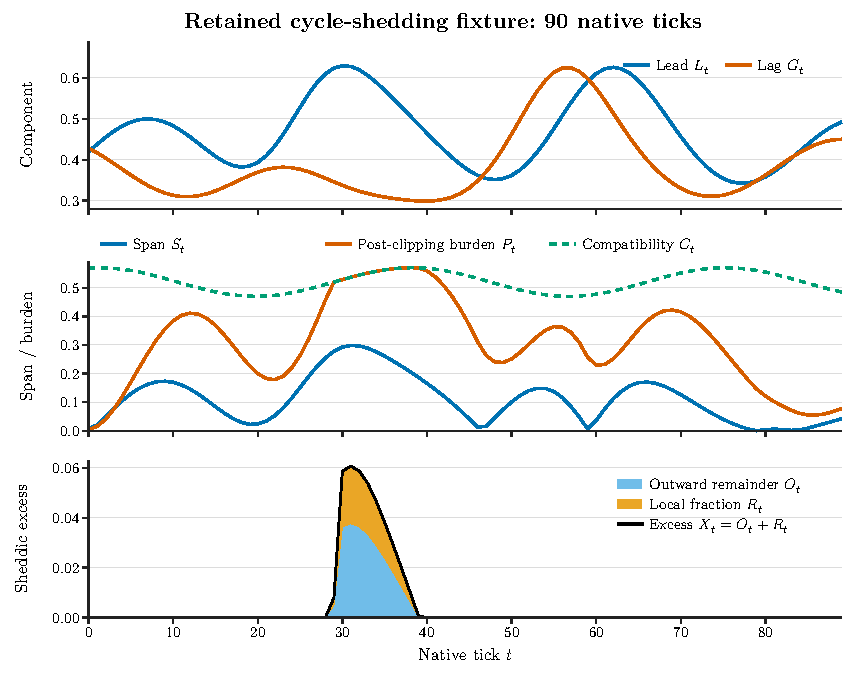
\includegraphics[width=0.92\linewidth,height=0.78\textheight,keepaspectratio]{figures/generated/cycle-disturbance-shedding-fixture.pdf}
\caption{Retained temporal-cycle fixture. The burden $P_t$ is post-clipping, with $P_t\le C_t$; the stacked outward and local fractions sum to $X_t$. Figure and summary use the same CSV. The summary label ``Total exoshedding'' denotes $\sum_tO_t$ in this fixture.}
\label{fig:v39-cycle-shedding-simulation}
\end{figure}

\begin{center}
% GENERATED FROM typst/manual/tables/cycle_shedding_summary.typ BY scripts/typ2tex.py (v1.0.0) — DO NOT EDIT.
% Edit canonical Typst under typst/ and regenerate with: python3 scripts/typ2tex.py --root . --outdir latex

{\small
\begin{tabular}{lr}
\toprule
Ticks & 90 \\
Maximum lead-lag span & 0.298 \\
Maximum temporal SADAR burden & 0.570 \\
Maximum sheddic excess & 0.061 \\
Total exoshedding & 0.238 \\
Total local reclosure & 0.146 \\
Sheddic path trigger ticks & 0 \\
First reclosure tick & none \\
\bottomrule
\end{tabular}
}

\end{center}

\subsection{Falsification}\label{manual:cycle-shedding-run-verdict}

If the computed values violate the stated recurrences on the declared ticks, the demonstration fails on that run.

\subsection{Data-support class reference}\label{manual:app:data-support-class-reference}

Manual fixtures and comparisons are read together with their declared data-support class. The compact class list is:

\[
\begin{array}{l|l}
D0 & \text{exact internal fixture}, \\
O0 & \text{observable-map fixture}, \\
G0 & \text{radial shell projection}, \\
G1 & \text{radial-medium projection}, \\
G2 & \text{three-dimensional field-dynamics retention}, \\
G3 & \text{time-resolved tracer-current simulation}, \\
L0 & \text{exact lensing toy fixture}, \\
L1 & \text{radial lens-medium diagnostic}, \\
L2 & \text{target-acquisition lane}, \\
L3 & \text{full lensing release class}.
\end{array}
\]

Errors and residuals are scoped to the class: $\delta_3$ for exact internal comparators, observable-map residuals for O0, radial square-speed residuals for G0/G1, retention and field residuals for G2/G3, and target-side residuals for L2/L3 after prediction values freeze.

\subsection{Audit}\label{manual:simfix:falsification}

Fixture audit records signed direction, scalar pressure, scope cancellation inside its declared boundary/window, and $\mathcal{E}(R,B)$ for a declared Stokes-valid scope.

\aodprovenance{\mainequation{main:eq:b-scoped-flux}; \mainequation{main:eq:sadar-attention-vector}; \mainequation{main:eq:stokes-audit-residual}; \mainappendix{main:app:scoped-flux-cancellation}; \mainappendix{main:app:combinatorics-rd-tests}.}

\subsection{Prediction-test placement}

Prediction tests and any collision-window comparison context belong in this manual scaffold. Application labels and external comparison records are carried by this manual scaffold. The main A$\Omega$D note supplies the AF/AFC/A$\Omega$D calculus and internal form names.

\subsection{Five-boundary exact rational cycle-shedding D.E.C. ledger}\label{manual:simfix:exact-rational-dec}

Declare the four-tick cycle-disturbance shedding stack

\[
B_{\mathrm{span}}\to B_{\mathrm{clip}}\to B_{\mathrm{shed}}\to B_{\mathrm{split}}\to B_{\mathrm{ext}}.
\]

Whereas the immutable summary table above displays rounded six-decimal coordinates, vector \texttt{RC-043} (\texttt{manual/data/boundary\_sadar/cycle\_shedding\_exact\_rational\_summary.csv}, verified by \texttt{python3 -B -m manual.engine} \texttt{--sector} \texttt{boundary\_sadar} and \texttt{aod-core} \texttt{--verify-vectors} \texttt{--check-zero-float}) evaluates every tick in exact rational arithmetic: $P_t=\min(B_t,C_t)$, shedding surplus $X_t=\max(0,B_t-C_t)$, outward fraction $O_t=(31/50)X_t$, and local retention $R_t=(19/50)X_t$, satisfying $O_t+R_t=X_t$ identically at every tick.

\begin{table}[H]
\centering
\caption{Exact rational four-tick cycle-disturbance clipping and $31/50$ versus $19/50$ shedding split D.E.C. ledger (\texttt{RC-043}).}
\label{tab:manual-app-a-exact-shedding-dec}
{\footnotesize
\begin{tabular}{rrrrrrrr}
\toprule
Tick & Span & Before clip $B_t$ & $C_t$ & Clipped $P_t$ & Shed $X_t$ & Outward $O_t$ & Local $R_t$ \\
\midrule
0 & $1/125$ & $11/2500$ & $14/25$ & $11/2500$ & 0 & 0 & 0 \\
1 & $29/50$ & $20163/62500$ & $1/4$ & $1/4$ & $2269/31250$ & $70339/1562500$ & $43111/1562500$ \\
2 & $7/10$ & $59/100$ & $1/4$ & $1/4$ & $17/50$ & $527/2500$ & $323/2500$ \\
3 & $1/20$ & $93/400$ & $3/10$ & $93/400$ & 0 & 0 & 0 \\
\bottomrule
\end{tabular}
}
\end{table}
